\documentclass[11pt, a4paper]{article}

\usepackage[utf8]{inputenc}
\usepackage[norsk]{babel}
\usepackage{amsmath, amssymb, amsfonts, amsthm}
\usepackage{bbm}
\usepackage{graphicx}
\usepackage{verbatim}
\usepackage{caption}
\usepackage{subcaption}
\usepackage{subfig}
\usepackage{float}

\newcommand{\vb}{\mathbf}

\addto{\cationsnorsk}{
  \renewcommand{\contentsname}
    {Innhald}
}

\addto{\cationsnorsk}{
  \renewcommand{\abstractname}
    {Samandrag}
}

\begin{document}

\begin{titlepage}

  \title{\normalsize FYS1120 Elektromagnetisme\\
    \vspace{10mm}
    \huge Labøving\\
    \vspace{10mm}
    \normalsize{\bf Hall-effekt.}}

  \author{Øyvind Sigmundson Schøyen}
%  \vspace{10mm}
%  \author{Kristian}
%  \vspace{10mm}
%  \author{Hilde Solesvik Skeie}

\end{titlepage}

\maketitle

\begin{abstract}
  Sei noko her.
\end{abstract}

\newpage
  \tableofcontents
\newpage

\section*{Oppgåve 1}
\addcontentsline{toc}{section}{Oppgåve 1}

  \subsection*{PRELAB-Oppgåve 1}
  \addcontentsline{toc}{subsection}{PRELAB-Oppgåve 1}
    Me vil lage eit program som tek imot datapunkter $x$ og $y$ og gjer oss eit plott over punkta mot eit polynom som interpolerer dei. \\ \\
    Eg har nytta Python kor metodane $\texttt{polyval}$ og $\texttt{polyfit}$ ligg i numpy-biblioteket. Me er då interesserte i eit program som les datapunkt frå ei fil
    og prøver å finne eit polynom som gjer oss ein god modell.
    \verbatiminput{\string~/Documents/3.Semester/FYS1120/Lab/Hall-effekt/src/PRELABOppgave1.py}

  \subsection*{Oppgåve 1.1}
  \addcontentsline{toc}{subsection}{Oppgåve 1.1}
    Me vil bestemme retningen til $\vb{B}$ og retningen til straumen gjennom prøven (p-Ge). Me lager ei skisse som viser Hall-spenninga sin polaritet.
    Deretter måler me Hall-spenninga $V_{H}$ som ein funksjon av $B$ ved konstant $I$. \\ \\
    Me byrjar med å sette opp måleinstrumenta som består av to straumforsyningar, eit amperemeter, eit voltmeter og ein spole for å lage eit magnetfelt.
    Me stiller på straumforsyninga til me får $I \approx 24.132$ A gjennom komponenten (p-Ge). Då stiller me på potmeteret til me måler $V = 0$ gjennom komponenten.



\newpage


\section*{Oppgåve 2}
\addcontentsline{toc}{section}{Oppgåve 2}

  \subsection*{PRELAB-Oppgåve 2.1}
  \addcontentsline{toc}{subsection}{PRELAB-Oppgåve 2.1}
    Me vil vise at straumtettheten $j$ er identisk med magnetiseringa $M$. \\ \\
    Det enklaste er å sjå på einingane til $j$ og $M$. Me får
    \begin{align*}
      j = \frac{dI}{dx} = \frac{I}{t} \sim \frac{\text{A}}{\text{m}},
    \end{align*}
    kor straumen $I$ er målt i Ampere og distansen $dx$ er gjeve i meter. $M$ er gjeve som magnetisk moment per volumeining. Då får me
    \begin{align*}
      M = \frac{\vb{\mu}}{V} = \frac{IA}{V} = \frac{I\pi a^2}{\pi a^2t} = \frac{I}{t} \sim \frac{\text{A}\text{m}^2}{\text{m}^3} = \frac{\text{A}}{{m}}.
    \end{align*}
    I tillegg til å få dei same einingane veit me at me jobber med dei same ``metrane''.

  \subsection*{PRELAB-Oppgåve 2.2}
  \addcontentsline{toc}{subsection}{PRELAB-Oppgåve 2.2}
    Vis at me ved å integrere opp overflatestraumen kan skrive magnetfeltet som
    \begin{align*}
      B_x(h) = \frac{\mu_0}{2}j\left[ \frac{h + t}{\sqrt{(h + t)^2 + a^2}} - \frac{h}{\sqrt{h^2 + a^2}} \right].
    \end{align*} \\ \\
    Me set inn uttrykket for straumen $I$ i uttrykket for $B_x(x)$.
    \begin{align*}
      j = \frac{dI}{dx} \qquad \Rightarrow \qquad I = j\ dx
    \end{align*}
    Då får me 
    \begin{align*}
      B_x &= \frac{\mu_0}{2}I \frac{a^2}{(x^2 + a^2)^{3/2}} \\
      &= \frac{\mu_0}{2}j\frac{a^2}{(x^2 + a^2)^{3/2}}\ dx \\
      &= \frac{\mu_0}{2}ja^2\int_h^{h + t}\frac{dx}{(x^2 + a^2)^{3/2}} \\
      &= \frac{\mu_0}{2}ja^2\left[ \frac{x}{a^2\sqrt{x^2 + a^2}} \right]_h^{h + t} \\
      &= \frac{\mu_0}{2}j\left[ \frac{h + t}{\sqrt{(h + t)^2 + a^2}} - \frac{h}{\sqrt{h^2 + a^2}} \right].
    \end{align*}

  \subsection*{PRELAB-Oppgåve 2.3}
  \addcontentsline{toc}{subsection}{PRELAB-Oppgåve 2.3}
    I denne oppgåven vil me teste programmet frå $\textbf{PRELAB-Oppgåve 1}$ med likninga frå $\textbf{PRELAB-Oppgåve 2.2}$.
    Me vil nytte 5-6 punkter for $t = 35$ mm og $a = 20$ mm. \\ \\
    Fyrst finner me vakuum permeabiliteten $\mu_0 = 4\pi \times 10^{-7}$ Vs/(Am) frå læreboka. For å finne $j$ nyttar me resultatet frå $\textbf{PRELAB-Oppgåve 2.1}$.
    \begin{align*}
      j = M = \frac{IA}{V} = \frac{I\pi a^2}{\pi a^2t} = \frac{I}{t}.
    \end{align*}
    kor straumen $I$ vert valgt til $I = 0.1$ A. Me får då resultatet
    \begin{figure}[H]
      \centering
      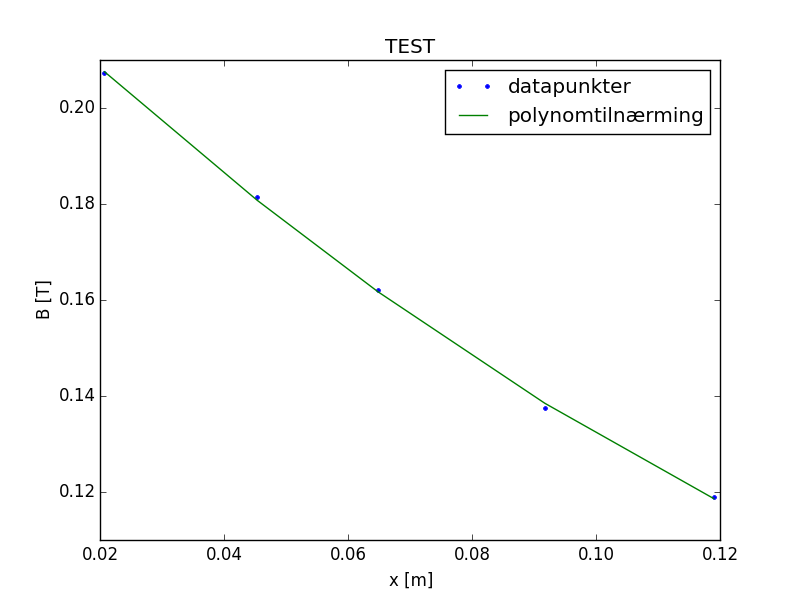
\includegraphics[width=400px]{\string~/Documents/3.Semester/FYS1120/Lab/Hall-effekt/src/PRELAB3.png}
      \caption{Her kan me sjå korleis polyfit prøver å tilpasse eit polynom til 6 punkter. Desverre vil det for så få punkter vere vanskeleg å gje eit nøyaktig resultat.}
    \end{figure}
    og utskrifta;
    \verbatiminput{\string~/Documents/3.Semester/FYS1120/Lab/Hall-effekt/src/Oppgave3.txt}
    Programmet $\texttt{PRELABOppgave3.py}$ er gjeve ved;
    \verbatiminput{\string~/Documents/3.Semester/FYS1120/Lab/Hall-effekt/src/PRELABOppgave3.py}

  \subsection*{PRELAB-Oppgåve 2.4}
  \addcontentsline{toc}{subsection}{PRELAB-Oppgåve 2.4}
    Me er interesserte i å sjå på $B$-feltet i topp-flata av magneten og når $t \to \infty$. Då lurer me og på kva $B$-feltet midt i sylinderen vert for noko. \\ \\
    Me startar med å sette inn $h = 0$ for å finne $B$-feltet i topp-flata. Me får
    \begin{align*}
      B_x(0) &= \frac{\mu_0}{2}j\left[ \frac{t}{\sqrt{t^2 + a^2}} - 0 \right] \\
      &= \frac{\mu_0}{2}\frac{tj}{\sqrt{t^2 a^2}}.
    \end{align*}
    For $t \to \infty$ får me
    \begin{align*}
      \lim_{t \to \infty} B_x(h) &= \lim_{t \to \infty} \frac{\mu_0}{2}j\underbrace{\left[ \frac{t}{\sqrt{t^2}} - \frac{h}{\sqrt{h^2 + a^2}} \right]}_{\approx 1} \\
      &= \frac{\mu_0}{2}j.
    \end{align*}
    Midt i sylinderen har me at $h = -\frac{t}{2}$ det gjer oss
    \begin{align*}
      B_x(-\frac{t}{2}) &= \frac{\mu_0}{2}j\left[ \frac{t}{2\sqrt{(t/2)^2 + a^2}} + \frac{t}{2\sqrt{(-t/2)^2 + a^2}} \right] \\
      &= \frac{\mu_0}{2}\frac{t}{\sqrt{(t/2)^2 + a^2}}.
    \end{align*}


\end{document}
